\section{Two-Body Problem$^\ast$ \label{ss:twobody}}

We examine the motion and orbit of the planet–star system. Treating both the planet and the star as point masses ($m_1$, $m_2$) with positions ${\boldsymbol{r_1}},{\boldsymbol{ r_2}}$, and assuming that the only force acting between them is gravity, the system reduces to the two-body problem, which can be solved analytically. Defining ${\boldsymbol{ r}} \equiv {\boldsymbol{r_2}} - {\boldsymbol{ r_1}}$ as in Fig.~\ref{fig:zahyou}, we introduce a polar coordinate system in the orbital plane with basis vectors ${\bf e}_r=(\cos{\theta}, \sin{\theta})^\top$ and ${\bf e}_\theta=(-\sin{\theta}, \cos{\theta})^\top$. Then ${\bf r} = r {\bf e}_r$, and with $\dot{{\bf e}}_r=\dot{\theta} (-\sin{\theta}, \cos{\theta})^T = \dot{\theta} {\bf e}_\theta $ and $\dot{{\bf e}}_\theta=\dot{\theta}(-\cos{\theta}, -\sin{\theta})^T = - \dot{\theta} \,\dot{{\bf e}}_r$, we obtain
\begin{align}
\label{eq:speconv1}
\dot{\bf r} = \frac{d}{dt}{r {\bf e}_r} = \dot{r} {\bf e}_r + r \dot{{\bf e}}_r = \dot{r} {\bf e}_r + r \dot{\theta} {\bf e}_\theta \\
\ddot{\bf r} = (\ddot{r} - r \dot{\theta}^2 ) {\bf e}_r + \left[ \frac{1}{r} \frac{d}{dt} (r^2 \dot{\theta} ) \right] {\bf e}_\theta .
\end{align}

Because $\boldsymbol{r_1}=-m_2/(m_1+m_2) \, \rv, \, \boldsymbol{r_2}= m_1/(m_1 + m_2) \,\rv$, the Lagrangian, with the barycenter at the origin and using the reduced mass $\mu = (m_1^{-1} + m_2^{-1})^{-1}$, is
\begin{align}
L &= T - U = \frac{m_1}{2} |\dot{\boldsymbol{r_1}}|^2 + \frac{m_2}{2} |\dot{\boldsymbol{r_2}}|^2 + G \frac{m_1 m_2}{r} \nonumber \\
&= \frac{\mu}{2} [ \dot{r}^2 + (r \dot{\theta})^2 ] + G \frac{m_1 m_2}{r}.
\end{align}

\begin{figure}[]
 \begin{center}
	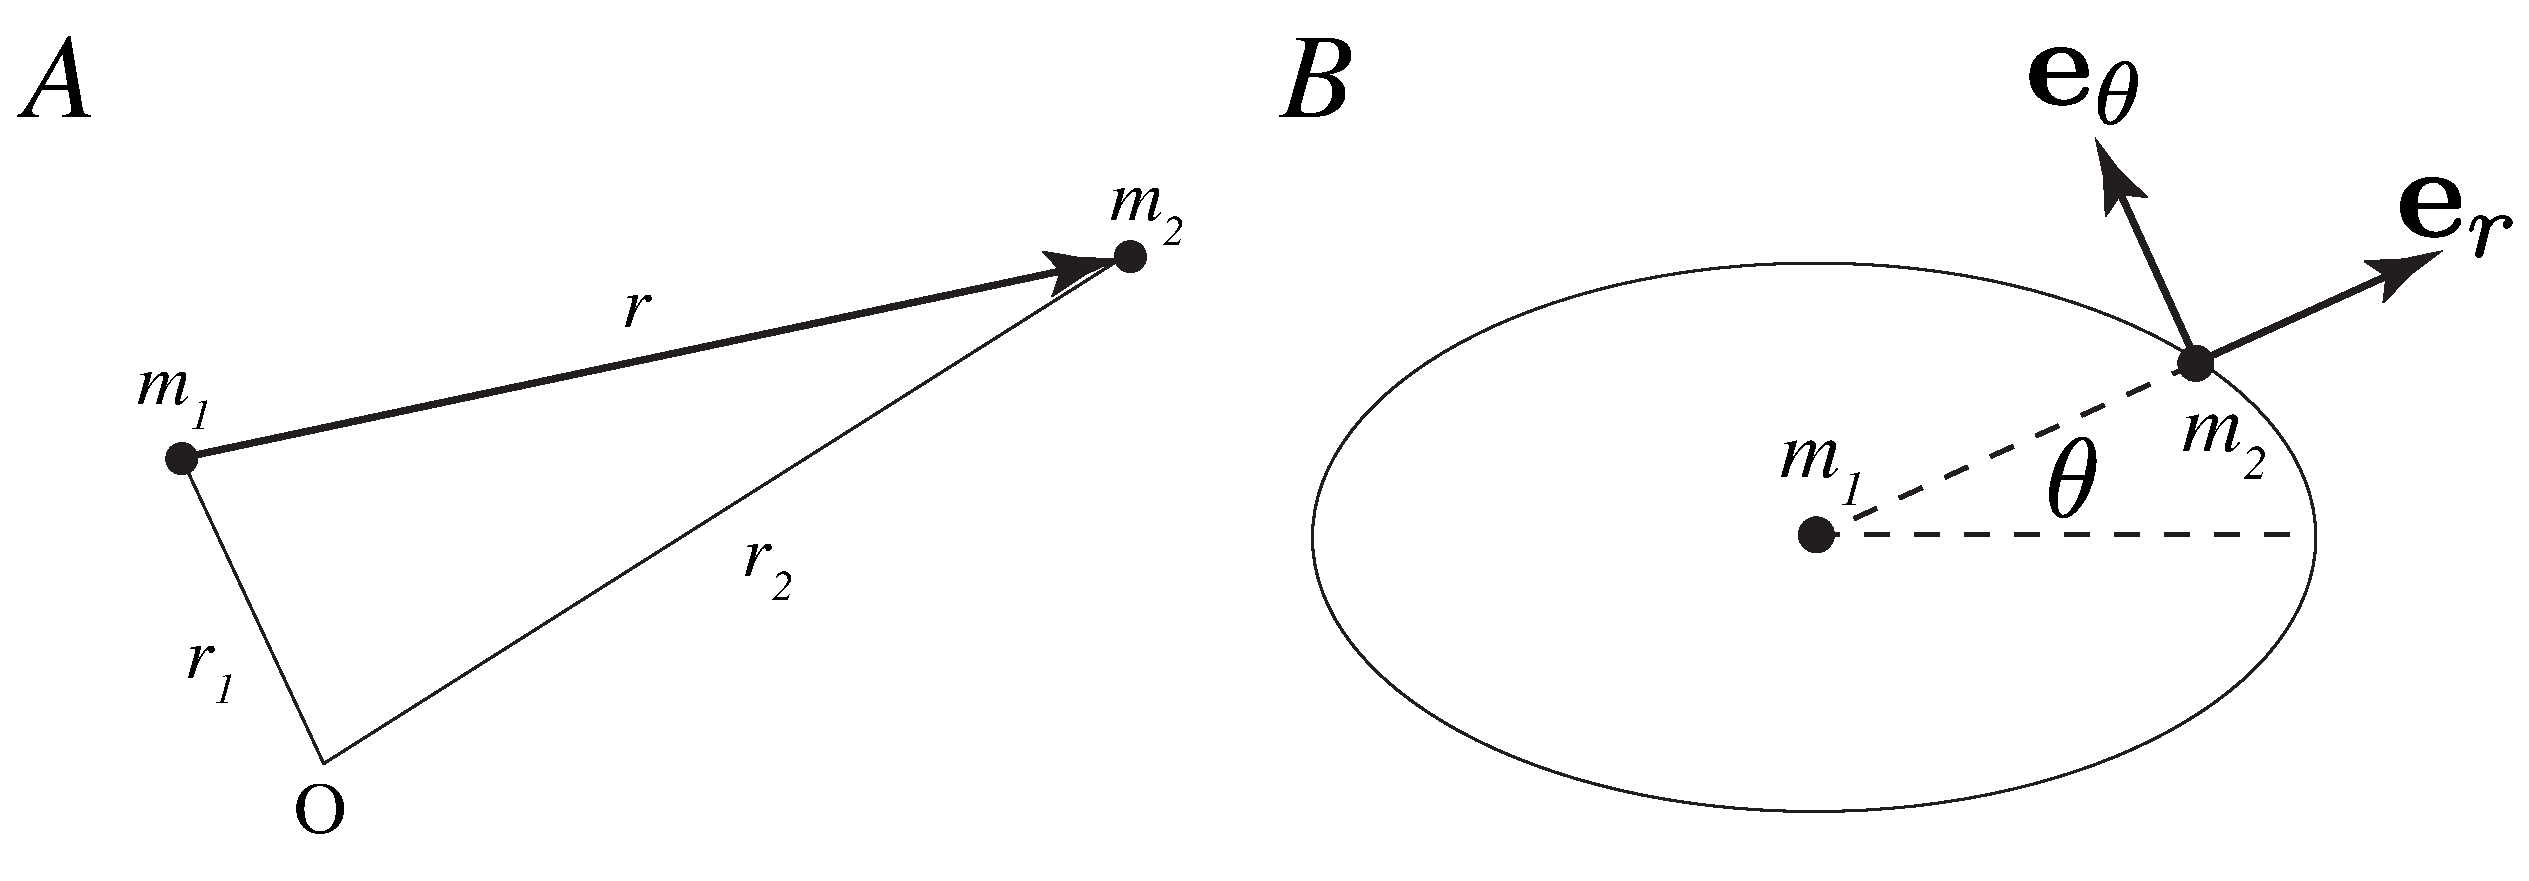
\includegraphics[width=\linewidth]{fig/zahyou.eps}
\end{center}
	\caption{Coordinate system}
	\label{fig:zahyou}
\end{figure} 


\color{red}
\begin{itembox}{Problem}
\footnotesize
\color{gray}
Derive 
\begin{align}
\label{eq:eqrad}
 \ddot{r} - r \dot{\theta}^2 = - \frac{G (m_1+m_2)}{r^2}
\end{align}
and $\dot{\bf h} =  0$ from the Lagrange equations
\begin{align}
\frac{d}{dt} \left( \frac{\partial L}{\partial \dot{r}}\right) - \frac{\partial L}{\partial r} = 0, \,\,\,
\frac{d}{dt} \left( \frac{\partial L}{\partial \dot{\theta}}\right) - \frac{\partial L}{\partial \theta} &= 0, 
\end{align}
where
$
{\bf h} \equiv {\bf r} \times \dot{\bf r} 
$
is the angular momentum vector. That is, the orbital angular momentum vector ${\bf h}$ is a conserved quantity in the two-body problem. This means that the point mass is constrained to move on the plane orthogonal to ${\bf h}$ (the orbital plane).
\end{itembox}
\color{black}

Transforming the variables in Eq.~(\ref{eq:eqrad}), let $u \equiv 1/r$. Using $h u^2 = \dot{\theta}$ and $\dfrac{d r}{d t} = \dfrac{d r}{d \theta} h u^2 = - h \dfrac{d u}{d \theta}$, we obtain
\begin{align}
\frac{d^2 u}{d \theta^2} + u = \frac{G (m_1 + m_2)}{h^2}
\end{align}
This is a nonhomogeneous second-order differential equation, whose homogeneous solution can be written as
\begin{align}
u_h = c_1 \cos{\theta} + c_2 \sin{\theta} = C_1 \cos{(\theta - C_2)} .
\end{align}
The nonhomogeneous solution is clearly
\begin{align}
u_i = \frac{G (m_1 + m_2)}{h^2} ,
\end{align}
and the general solution is the sum of these. Factoring out $G (m_1 + m_2)/h^2$ and introducing integration constants $e$ and $\omega$, the general solution can be written as
\begin{align}
u = \frac{G (m_1 + m_2)}{h^2} [ 1 + e \cos{(\theta - \omega)}] .
\end{align}
Returning to $r=1/u$, we obtain
\begin{align}
\label{eq:eqkep}
r = \frac{h^2}{G (m_1 + m_2)} \frac{1}{ 1 + e \cos{(\theta - \omega)}} .
\end{align}

Now, let us consider an ellipse as in Fig.~\ref{fig:ellip}. For an ellipse,
\begin{align}
\label{eq:rellp}
r + r^\prime = 2 a
\end{align}
holds. From the coordinates, we have
\begin{align}
\label{eq:rellp2}
(r^\prime)^2 &= (x_p + 2 e a )^2 + y_p^2 \nonumber \\
&= (r \cos{\theta} + 2 e a )^2 + (r \sin{\theta})^2 ,
\end{align}
and eliminating $r^\prime$ from Eqs.~(\ref{eq:rellp},\ref{eq:rellp2}), we obtain the conic equation of the ellipse
\begin{align}
\label{eq:conic_orig}
r = \frac{a (1-e^2)}{ 1 + e \cos{\theta}} .
\end{align}


\begin{figure}[]
 \begin{center}
	\includegraphics[bb=0 0 695 428,width=1.0\linewidth]{fig/ellip.png}
% \includegraphics[bb=0 0 474 461,width=1.0\linewidth]{fig/orbele.png}
\end{center}
	\caption{Ellipse.}
	\label{fig:ellip}
\end{figure} 

Defining the semi-major axis $a$, the semi-minor axis $b$, and the true anomaly $f$ as
\begin{align}
\label{eq:defkeppar1}
\frac{h^2}{G (m_1 + m_2)} &= a (1 - e^2) \\
\label{eq:defkeppar2}
b^2 &= a^2 (1 - e^2) \\
\label{eq:defkeppar3}
f &\equiv \theta - \omega ,
\end{align}
Eq.~(\ref{eq:eqkep}) takes the form of the conic equation
\begin{align}
\label{eq:conic_kepler}
r = \frac{a (1-e^2)}{ 1 + e \cos{f}} ,
\end{align}
which confirms that the solution of the two-body problem is an ellipse (with $0 \le e < 1$). The true anomaly $f$ corresponds to the angle of the star–planet system measured from the periastron (the point closest to the star, analogous to the solar periastron). The quantity $\omega$ is called the argument of periastron and represents a counterclockwise rotation of the ellipse described by the conic equation (\ref{eq:conic_orig}) by an angle $\omega$.

Since $\dot{A}$ is constant, the area of the ellipse can be written as
\begin{align}
A = \pi a b = \frac{h}{2} P ,
\end{align}
where $P$ is the orbital period. Rearranging this expression, we obtain
\begin{align}
\label{eq:kep3}
P^2 = \frac{4 \pi^2}{G (m_1+m_2)} a^3 ,
\end{align}
which shows that the square of the orbital period is inversely proportional to the total mass and proportional to the cube of the semi-major axis (Kepler’s third law). In the case of a circular orbit, the orbital angular velocity is given by $1/\sqrt{G (m_1+m_2) a}$. Eliminating $G$ using Eq.~(\ref{eq:defkeppar1}), we also obtain an expression in terms of angular momentum,
\begin{align}
\label{eq:kep3_1}
P = \frac{2 \pi a^2 \sqrt{1-e^2}}{h} .
\end{align}

\begin{figure}[]
 \begin{center}
%	\includegraphics[bb=0 0 695 428,width=1.0\linewidth]{fig/ellip.png}
 \includegraphics[bb=0 0 474 461,width=1.0\linewidth]{fig/orbele.png}
\end{center}
	\caption{Coordinate system.}
	\label{fig:ellip}
\end{figure} 

The mean motion is defined by
\begin{align}
    n \equiv \frac{2 \pi}{P}.
\end{align}
From equation (\ref{eq:kep3_1}), we can also express the mean motion as
\begin{align}
\label{eq:mean_motion}
    n = \frac{h}{a^2 \sqrt{1-e^2}}.
\end{align}


\section{Two-body problem in three-dimensional space \label{ss:threedtwobody}}

In the previous chapter, we considered two-body motion on a two-dimensional plane. In reality, celestial bodies exist in three-dimensional space from the perspective of an observer, so the orbit must be rotated into 3D. The orbital inclination $i$, which represents the tilt relative to the observer, and the longitude of the ascending node $\Omega$, which specifies the azimuthal direction, are introduced. By specifying the six parameters $a, e, \omega, f, i, \Omega$, the orbit of the two-body problem in three-dimensional space is uniquely determined.

Let us represent these rotations using rotation matrices. First, we take the reference ellipse to be that described by the conic equation (\ref{eq:conic_orig}) and shown in Fig.~\ref{fig:ellip}. The $z$-axis is taken perpendicular to the plane of the page.
\begin{itemize}
\item (1) Rotating the conic equation (\ref{eq:conic_orig}) counterclockwise about the $z$-axis by $\omega$ gives the ellipse of the two-body problem, Eq.~(\ref{eq:conic_kepler}).
\item (2) Next, rotating counterclockwise about the $x$-axis by $i$ tilts the orbital plane by $i$ with respect to the celestial sphere. 
\item (3) Finally, a remaining degree of freedom corresponds to rotation about the $z$-axis by $\Omega$, namely the azimuthal rotation on the celestial sphere.
\end{itemize}

Applying these rotation matrices in sequence to the vector representing the ellipse $\rv = (r \cos{\theta}, r \sin{\theta},0)$, we first obtain (1):

% ---- 1. position in the orbital plane ---------------------------------
\begin{align}
\rv &=
\begin{pmatrix}
r\cos\theta\\
r\sin\theta\\
0
\end{pmatrix}
=
\begin{pmatrix}
r\cos\!\bigl(f+\omega\bigr)\\
r\sin\!\bigl(f+\omega\bigr)\\
0
\end{pmatrix}
.
\end{align}
Next, (2) is 
% ---- 2. rotation by the inclination i (about the x-axis) --------------
\begin{align}
\rv^\prime &=
\begin{pmatrix}
1 & 0        & 0\\
0 & \cos i   & -\sin i\\
0 & \sin i   &  \cos i
\end{pmatrix}
\rv \\
&=
\begin{pmatrix}
r\cos\!\bigl(f+\omega\bigr)\\
r\sin\!\bigl(f+\omega\bigr)\cos i\\
r\sin\!\bigl(f+\omega\bigr)\sin i
\end{pmatrix}
.
\end{align}

% ---- 3. rotation by the longitude of ascending node Ω (about the z-axis)
Lastly, we obtain the trajectory in the three-dimensional space $(X,Y,Z)$ from (3):  
\begin{align}
\rv^{\prime\prime} &=
\begin{pmatrix}
\cos\Omega & -\sin\Omega & 0\\
\sin\Omega &  \cos\Omega & 0\\
0          &  0          & 1
\end{pmatrix}
\rv^\prime \\
&=
\begin{pmatrix}
r\cos\!\bigl(f+\omega\bigr)\cos\Omega
 - r\sin\!\bigl(f+\omega\bigr)\cos i\,\sin\Omega\\[4pt]
r\cos\!\bigl(f+\omega\bigr)\sin\Omega
 + r\sin\!\bigl(f+\omega\bigr)\cos i\,\cos\Omega\\[4pt]
r\sin\!\bigl(f+\omega\bigr)\sin i
\end{pmatrix}
\\
\label{eq:threed}
&\equiv
\begin{pmatrix}
X\\[2pt] Y\\[2pt] Z
\end{pmatrix}.
\end{align}

\section{Two-body problem as a function of time}

The solution to the two-body problem has so far been expressed as a function of the true anomaly $f$, namely $r = r(f)$. However, in actual observations, the two-body problem is always observed as a function of time. We therefore consider how to obtain the time-dependent expression $r = r(t)$.

The approach is as follows. First,
\begin{align}
v^2 &= \dot{\rv} \cdot \dot{\rv}
= (\dot{r} {\ev}_r + r \dot{f} {\ev}_\theta) \cdot (\dot{r} {\ev}_r + r \dot{f} {\ev}_\theta) \nonumber \\
\label{eq:v2_1}
&= \dot{r}^2 + r^2 \dot{f}^2 \\
\label{eq:v2_2}
&= \dot{r}^2 + \frac{h^2}{r^2} ,
\end{align}
where we used $h = r^2 \dot{f}$. Then,
\begin{itemize}
\item (1) Express $v^2$ in terms of $f$ by transforming $r$ and $\dot{r}$ in Eq.~(\ref{eq:v2_2}), giving $v^2(f)$.
\item (2) Transform $v^2(f)$ into $v^2(r)$ using the conic equation.
\item (3) Equating $v^2 = \dot{r}^2 + h^2/r^2$, derive an equation for $r$ and $\dot{r}$, namely a differential equation for $r$ with respect to time.
\end{itemize}

For step (1), the transformation from $r$ to $f$ can be made using the conic equation (\ref{eq:conic_kepler}). To express $\dot{r}$ in terms of $f$, we use
\begin{align}
\label{eq:dotr}
\dot{r} &= \frac{h}{a(1-e^{2})} \, e\sin f .
\end{align}

\begin{itembox}{$\clubsuit$ Derivation of Equation (\ref{eq:dotr})}
\footnotesize
\color{gray}
\begin{align}
    \dot r
  &=\frac{df}{dt}
   \,\frac{d}{df}\!
     \left(
       \frac{a(1-e^{2})}{1+e\cos f}
     \right)
  =\dot f\,
    \frac{a(1-e^{2})\,e\sin f}{\bigl(1+e\cos f\bigr)^{2}}
    \nonumber \\
    &= \dot{f} \frac{a (1-e^2)}{1 + e \cos{f}} \frac{e \sin{f}}{1 + e \cos{f}} = r \dot{f} \frac{e \sin{f}}{1 + e \cos{f}} \nonumber\\
&= \frac{h}{r} \frac{e \sin{f}}{1 + e \cos{f}}
= \frac{h}{a(1-e^{2})}\,e\sin f
\end{align}
\end{itembox}

Then, we obtain
\begin{align}
    v^2 &= \dot{r}^2 + (r \dot{f})^2 = \dot{r}^2 + \frac{h^2}{r^2} \nonumber \\
    &= \frac{h^2}{a^2(1-e^2)^2} [2 (1 + e\cos{f}) + e^2 - 1 ] = v^2(f).
\end{align}


Next, step (2), where $v^2(f)$ is transformed back into a function of $r$ using the conic equation, gives
\begin{align}
v^2(r) &= \frac{h^2}{a (1 - e^2)} \left( \frac{2}{r} - \frac{1}{a} \right) .
\end{align}
From step (3), we obtain the time differential equation for $r$:
\begin{align}
\label{eq:rde}
\dot{r}^2 - \frac{h^2}{a (1-e^2)} \left( \frac{2}{r} - \frac{1}{a} \right) + \frac{h^2}{r^2} = 0 .
\end{align}
This equation cannot be solved directly. Therefore, we introduce the eccentric anomaly $E$:
\begin{align}
\label{eq:eanomaly}
r = a (1 - e \cos{E}) .
\end{align}
Using this $E$, we transform the differential equation (\ref{eq:rde}) into a differential equation in terms of $E$ and $\dot{E}$:
\begin{align}
\label{eq:dee}
\dot{E} = \frac{n}{1 - e \cos{E}} .
\end{align}
Although introduced somewhat ad hoc, the solution is given by
\begin{align}
E - e \sin{E} = n (t -t_0) ,
\end{align}
and one can verify Eq.~(\ref{eq:dee}) by differentiation. Here, defining the mean anomaly $M$ as a proxy for the time variable,
\begin{align}
M \equiv n (t - t_0),
\end{align}
we obtain
\begin{align}
\label{eq:dee_sol_M}
f(E) = E - e \sin{E} - M = 0 ,
\end{align}
whose solution yields $E$.

\begin{itembox}{$\clubsuit$ Derivation of Equation (\ref{eq:dee})}
\footnotesize
\color{gray}
\begin{align}
  \frac{2}{r}-\frac{1}{a}
    &=\frac{1}{a}\!\left(\frac{2}{1-e\cos E}-1\right)     \nonumber \\
    &=\frac{1}{a}\,\frac{1+e\cos E}{1-e\cos E}
      \;=\;
      \frac{1}{a}\,
      \frac{1-e^{2}\cos^{2}E}{(1-e\cos E)^{2}}\;.
\end{align}

\begin{align}
 &\frac{h^{2}}{r^{2}}
 -\frac{h^{2}}{a^{2}(1-e^{2})}\!
  \left(\frac{2}{r}-\frac{1}{a}\right) \nonumber \\
 &= \frac{h^{2}}{a^{2}(1-e\cos E)^{2}}
    -\frac{h^{2}(1-e^{2})}{a^{2}(1-e\cos E)^{2}(1-e^{2})} \nonumber \\
 &=\frac{h^{2}(1-e^{2})}{a^{2}(1-e\cos E)^{2}(1-e^{2})} -\frac{h^{2}(1-e^{2}\cos^{2}E)}{a^{2}(1-e\cos E)^{2}(1-e^{2})}\nonumber \\
 &= -\frac{h^{2}e^{2}\bigl(1-\cos^{2}E\bigr)}
        {a^{2}(1-e\cos E)^{2}(1-e^{2})}
\end{align}

\begin{align}
     \dot r &=\frac{dE}{dt}\,
         \frac{d}{dE}\bigl(a(1-e\cos E)\bigr)
     =\dot E\,a e\sin E \\
  \dot r^{2}
    &=\dot E^{2}\,a^{2}e^{2}\sin^{2}E
\end{align}

From these equations, we obtain
\begin{align}
    \dot E^{2}\,a^{2}e^{2}\bigl(1-\cos^{2}E\bigr)
  =
  \frac{h^{2}\,e^{2}\bigl(1-\cos^{2}E\bigr)}
       {a^{2}(1-e\cos E)^{2}(1-e^{2})},
\end{align}
that is,
\begin{align}
    \dot E^{2}
   =\frac{h^{2}}
          {a^{4}(1-e\cos E)^{2}(1-e^{2})}
\end{align}
Assuming $\dot{E} > 0$, we obtain
\begin{align}
    \dot E
 &=\frac{h}{a^{2}\sqrt{1-e^{2}}\,(1-e\cos E)} \\
 & = \frac{n}{1 - e \cos{E}}.
\end{align}

We used the representation of the mean motion (\ref{eq:mean_motion}).
\end{itembox}
Furthermore, the relationship between $E$ and $f$ can be derived from Eq.~(\ref{eq:eanomaly}) and the conic equation of the two-body problem (\ref{eq:conic_kepler}):
\begin{align}
\label{eq:Efrel}
\cos{f} = \frac{\cos{E} - e}{1 - e \cos{E}} .
\end{align}

Thus, once the period $P$ and the offset $t_0$ are known, the mean anomaly $M$ can be calculated from the time $t$. By solving Eq.~(\ref{eq:dee_sol_M}) numerically, one obtains $E$, and then the true anomaly $f$ can be determined from Eq.~(\ref{eq:Efrel}).\\

\subsubsection{Solving Eq.~(\ref{eq:dee_sol_M}) using the Newton–Raphson method}

The nonlinear equation $f(E)=0$ must be solved numerically. One method for doing so is the Newton–Raphson method. As illustrated in Fig.~\ref{fig:newton_raphson}, the procedure begins with an initial guess $E_1$, then determines the tangent line to $f(E)$ at $E_1$, and finds analytically the intersection of this line with the $E$-axis, which is taken as $E_2$. Repeating this procedure $n$ times yields successive approximations. At the $i$-th step, the tangent line (i.e., the first-order Taylor expansion of $f(E)$ about $E_i$) is
\begin{align}
\label{eq:nrm}
y = f(E_i) + f^\prime(E_i) (E - E_i) ,
\end{align}
and therefore,
\begin{align}
\label{eq:update_newton}
E_{i+1} &= E_i + \Delta E_i \\
\Delta E_i &\equiv - \frac{f(E_i)}{f^\prime(E_i)} .
\end{align}
Here, $\Delta E_i$ is called the update term at the $i$-th iteration\footnote{This can also be viewed simply as updating the solution using the first-order Taylor approximation of $f(E)$,
\begin{align}
\label{eq:nrm_f}
f(E) \approx f(E_i) + f^\prime(E_i) (E - E_i) = 0 ,
\end{align}
taking $E_{i+1}$ as the solution, and repeating the procedure.}. This iteration is repeated until the convergence criterion $|E_{i+1} - E_i| < \epsilon$ is satisfied, where $\epsilon$ is the tolerance, and the resulting $E_i$ is taken as the approximate solution.

For the calculation in Eq.~(\ref{eq:nrm}), the derivative of $f$ is required. From Eq.~(\ref{eq:dee_sol_M}),
\begin{align}
f^\prime(E) = 1 - e \cos{E} .
\end{align}


\begin{figure}[]
 \begin{center}
 \includegraphics[width=1.0\linewidth]{fig/newton_raphthon.png}
\end{center}
	\caption{Newton-Raphson method.}
	\label{fig:newton_raphson}
\end{figure} 

\begin{itembox}{Newton's method as 2nd-order optimization$^\dagger$}
\footnotesize
\color{gray}
Consider the optimization problem of finding $x = x^\ast$ that minimizes a cost function $Q(x)$:
\begin{equation}
x^\ast = \mathrm{minimize}_{x} \,\, Q(x) .
\end{equation}
The stationary condition
$d Q(x)/d x = 0$
can be solved using the Newton–Raphson method. In this case, by setting
$f (x) = Q^\prime (x)$
and applying Eq.~(\ref{eq:update_newton}), the update rule becomes
\begin{align}
x_{i+1} &= x_i + \Delta x_i \\
\Delta x_i &\equiv - \frac{Q^\prime (x_i)}{Q^{\prime\prime}(x_i)} ,
\end{align}
which requires the second derivative of $Q(x)$. For this reason, it is called second-order optimization. In the context of optimization, the term ``Raphson'' is usually omitted, and it is simply called Newton's method.

In general, the multidimensional version of Newton's method can be formulated in the same way. From the multidimensional Taylor expansion,
\begin{align}
\fv(\xv) \approx \fv(\xv_i) + \Jv (\xv_i) (\xv - \xv_i) = \boldsymbol{0},
\end{align}
the solution $\xv$ becomes the next update point, leading to
\begin{align}
\xv_{i+1} &= \xv_{i} + \Delta \xv_i \\
\label{eq:second_newton}
\Delta \xv_i &\equiv - \Jv^{-1} (\xv_i) \fv(\xv_i) ,
\end{align}
where $\Jv (\xv_i)$ is the Jacobian at $\xv_i$.
\end{itembox}

